
\section{RFI mitigation}\seclab{RFIm}

The purpose of \verb!"RFI_Mitigation.sh"! is to pre-process the data-files for a single flash and in the process determine the frequency notch filters to mitigate RFI. The RFI filter data is written to \verb!"Book/RFI_Filters.uft"! of the main flash-working directory `FlashFolder'. The file names to be processed are read from the file \verb!"directory.out"! (should be in the FlashFolder) as was created by the script \verb!"NewFlash.sh"!. The script \verb!"NewFlash.sh"! should have automatically started the running of \verb!"RFI_Mitigation.sh"!.


The files will be processed in the order as listed in \verb!"directory.out"!
where the \note{ second } station in the directory listing will be used as the reference station later in imaging (to change this replace the ``2" on the line \verb!"${ProgramDir}$Prog ${AntennaFieldsDir} 2"! by the appropriate number in \verb!"RFI_Mitigation.sh"!). Be careful to set here a station that is in a rather dense part of the array, preferably be it  CS002.

Additional axillary information needed for the imaging runs is written to\\ \verb!"Book/LOFAR_H5files_Structure.dat"! .

The script \verb!"RFI_Mitigation.sh"! takes a while to run. At the end it will submit the script \verb!Explore.sh!.


\subsection{Additional details}

All files in the directory listing given in \verb!"'directory.out'"! are scanned. If 9 of the first 100 data-chunks of a specific antenna are non-zero an RFI analysis is made otherwise the antenna is omitted from further analysis. The amplitudes of the 9 frequency spectra are summed. In the range of 25 to 79~MHz. A running (inclined) straight line fit is made over 2~MHz. When the amplitude is larger that the average (from the line-fit) that frequency is filtered out. In addition the power in this frequency range is determined as the sum of the square amplitude (in frequency). This power will later be used to normalize spectra. The antenna positions are obtained from the files in directory \verb!"AntennaFields/"! (in ``MainDir") and written to the auxiliary file.

\subsection{Figures and print-out}\seclab{RFI-out}


\begin{figure}[th]
\centering{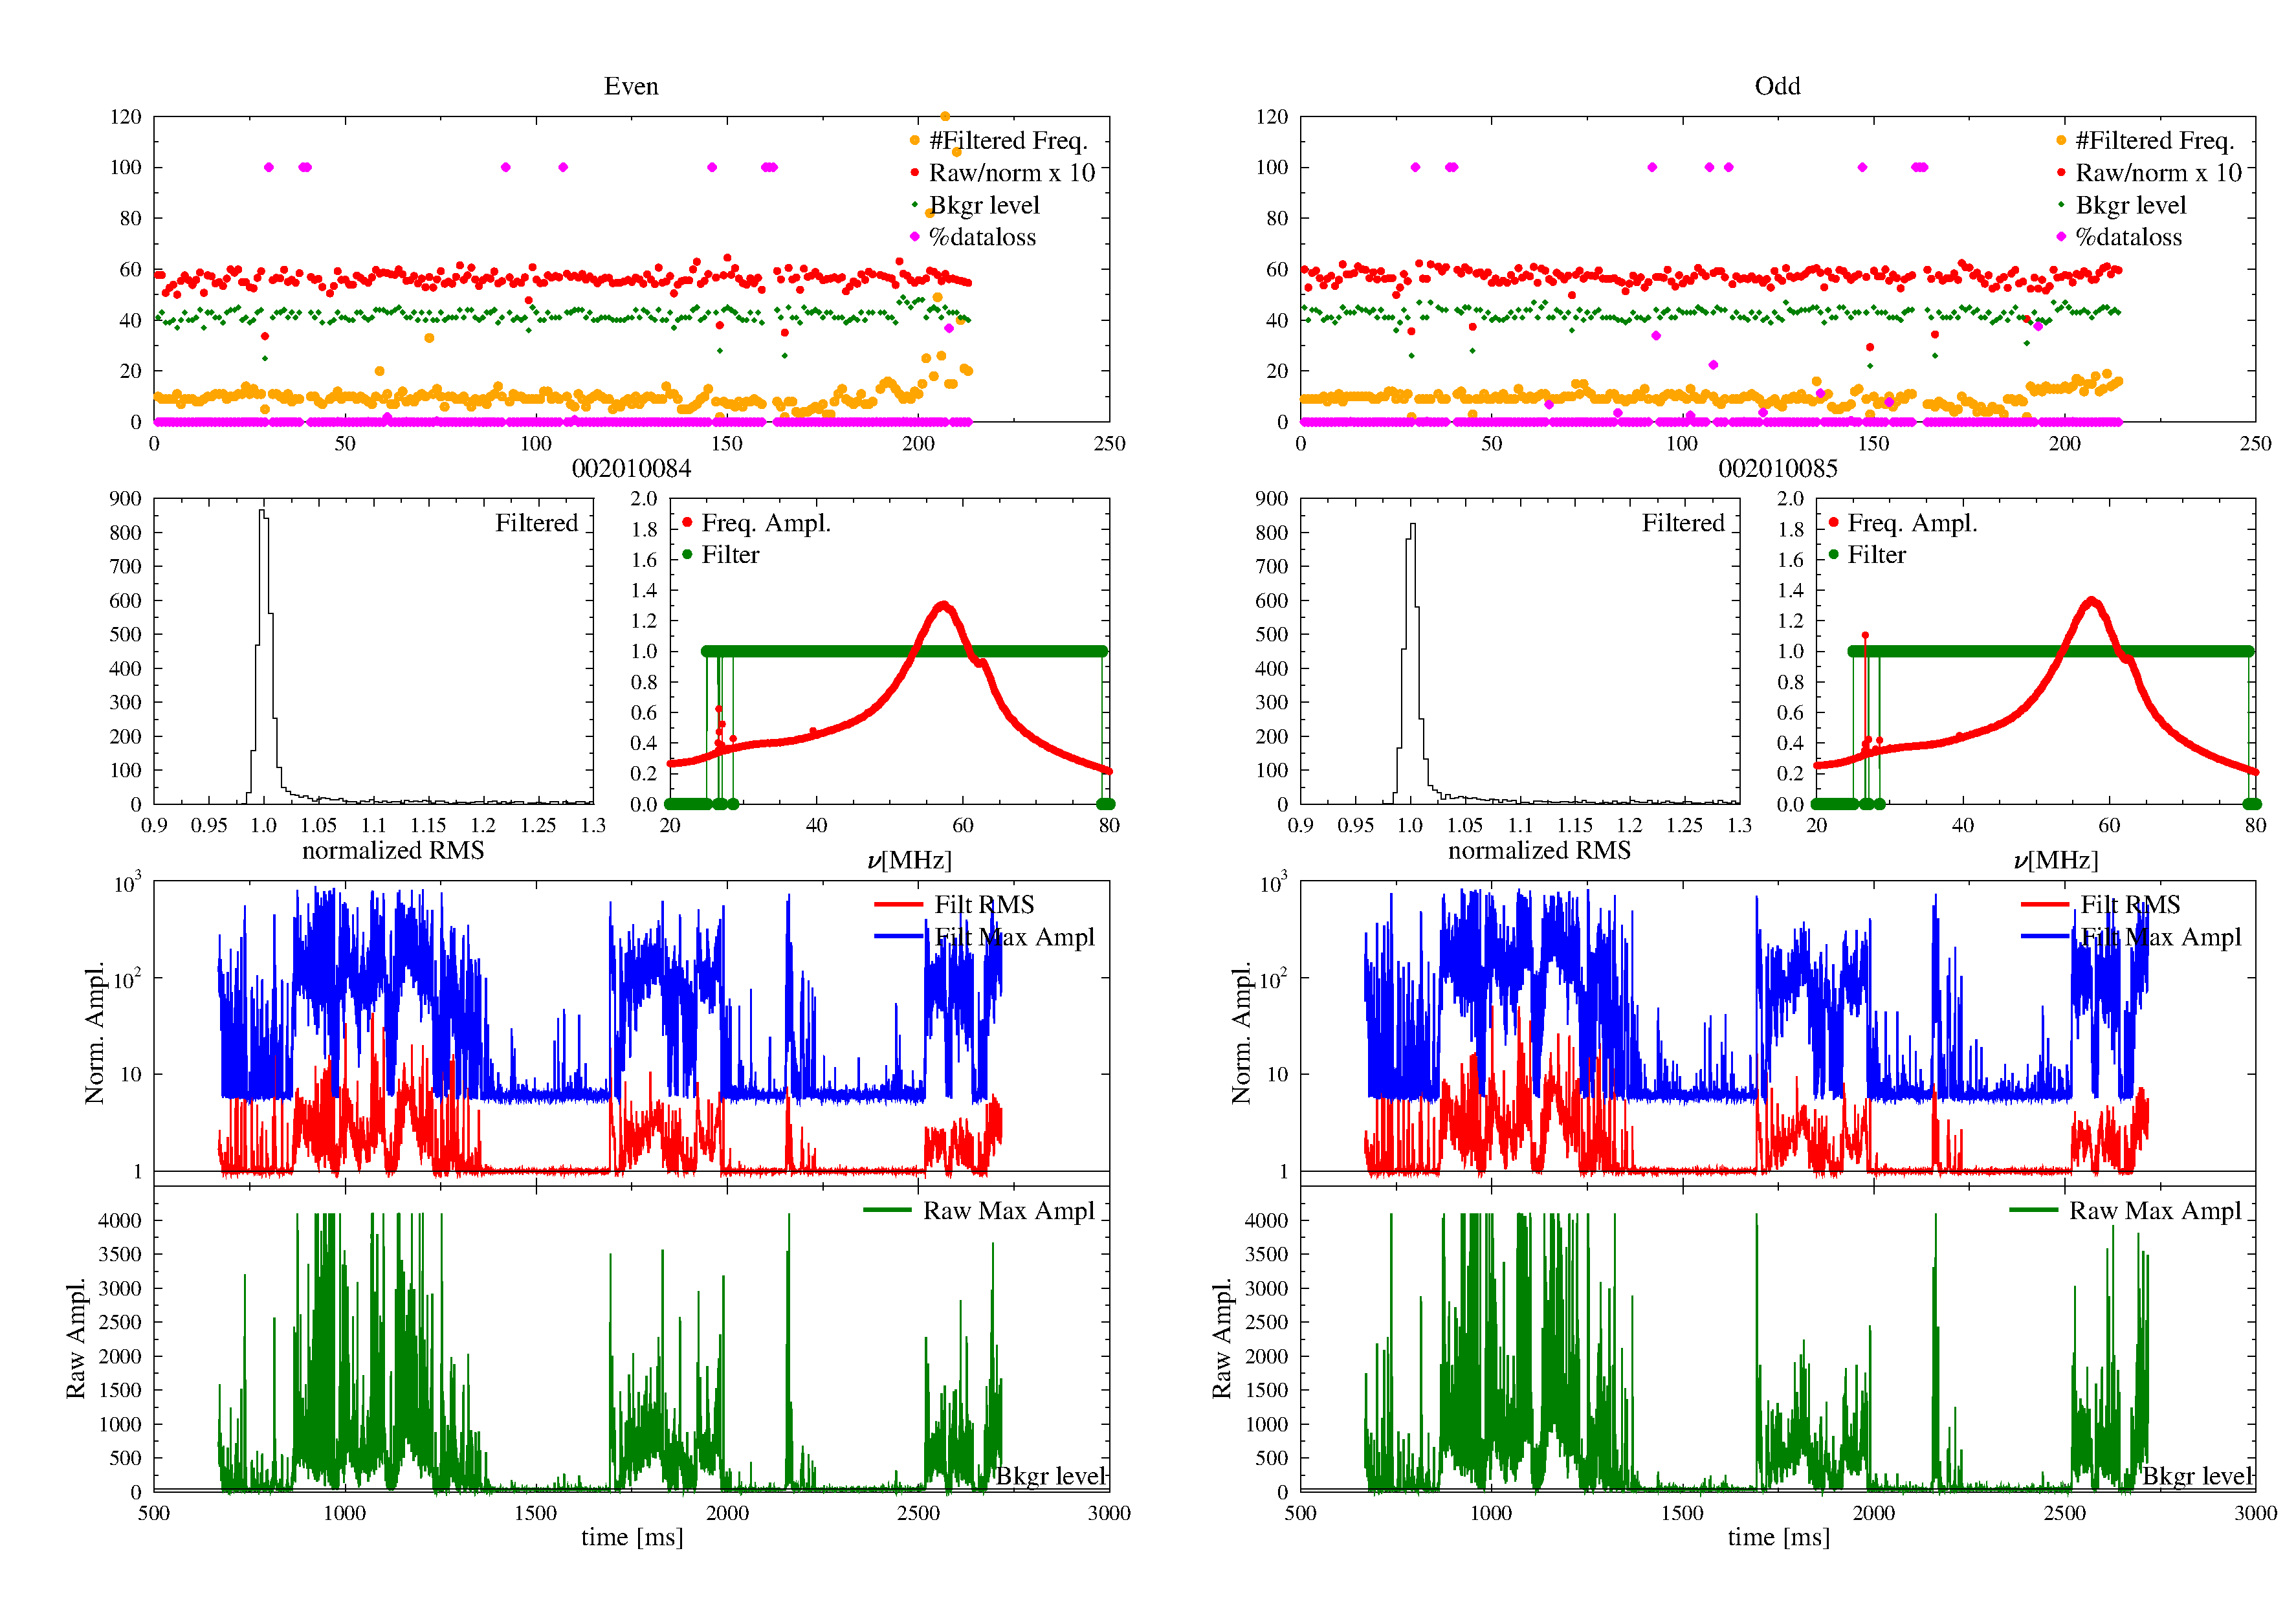
\includegraphics[width=0.89\textwidth]{Figs/RFI_Plots-20A7} }
%\centering{\includegraphics[ bb=1.0cm 2.4cm 24.5cm 25.7cm,clip, width=0.49\textwidth]{../Figs/SE20A7-NPMx_1HIntfSpecSel} }
	\caption{RFI plot results result for a typical flash, 20A-7 in this case.}	 \figlab{Intf-NLaH}
\end{figure}

In \figref{Intf-NLaH} a typical plot is shown as generated by the RFI-mitigation program. The results are presented separately for Even- (odd-) numbered antennas officially known as Y- (X-)dipoles. The to panel shows for each antenna (over 200 even and odd antennas for this case). For all values it is important that it does not vary too much, where outliers need to be scrutinized.
\begin{description}
\item[orange] The number of notch filters to mitigate RFI within the specified frequency band (30-80~MHz). The RFI filters are determined per antenna and taken the same for all data-chunks.
\item[red] The normalization factor between raw data and the noise-normalization.
\item[green] For every chunk of data (0.3~ms) the maximum amplitude is determined. The minimum value for all chunks of these maxima/chunk, a measure of the background, is shown.
\item[magenta] The percentage of data chunks that have too much data loss to be considered in the analysis.
\end{description}
The panel ``Filtered'' gives the Distribution of mean power (square of the complex amplitude) after filtering per chunk for all chunks in the reference station.
The panel next to it gives the frequency filter (for the reference station) in green and the antenna gain in red.

The bottom panels give, again for the reference antenna, for each chunk, the RMS power after RFI filtering (the same data as used in making the plot in panel ``filtered''), and the maximum amplitude (blue: after filtering, green: before filtering). This gives a good indication of the time-frames with lightning activity. Note that for this example the reference antenna had no data loss, if it had, the blue line would go to the bottom of the panel for the chunks with data loss.

Part a typical output (the .out file) that contains useful info for further imaging (the non-diagnostic part).

\begin{linenumbers}
\tiny
\resetlinenumber
\begin{verbatim}
 time range for which there are data [ms]   669.00223999999992        2717.0073600000001
 !!!!!!!!! For           22  Antennas RFI-mitigation failed, out of a total of         427  !!!!!!!!!!!!
        5094        5095        7093       11088       11089       11090       11091       13088       32086       32087      103092      103093      121091      125088      125089      130092      130093      130094      130095      145088      145089      166094
 MinAmp statistics:   41.883950617283951        41.991680539934350
 statistics powr=sq(raw/Norm):   31.767085498017074        31.995666167967695
 !!!!!!!! Bad antenna based on Raw Amplitude range        5092          25   32.866010868572779        50.901890365995122
 !!!!!!!! Bad antenna based on powr        5092          11
 !!!!!!!! Bad antenna based on Raw Amplitude range        5093          26   32.866010868572779        50.901890365995122
\end{verbatim}
\end{linenumbers}

This summary lists the antennas that are -most likely- better be omitted from subsequent analysis. Given is the Station Antenna ID (SAI) number that is used internally in the analysis code. The translation table from station ID to station Mnemonic is
{
\tiny
\begin{verbatim}
       1     2     3     4     5     6     7    11    13    17    21    24    26    28    30    32   103   106
   CS001 CS002 CS003 CS004 CS005 CS006 CS007 CS011 CS013 CS017 CS021 CS024 CS026 CS028 CS030 CS032 CS103 RS106

     121   125   128   130   141   142   145   146   147   150   161   166   167   169   181   183   188   189
   CS201 RS205 RS208 RS210 CS301 CS302 RS305 RS306 RS307 RS310 CS401 RS406 RS407 RS409 CS501 RS503 RS508 RS509
\end{verbatim}
}
The (most often) long line with numbers are the SAI of stations where the RFI-suppression filter could not be determined due to too much data loss. The following lines give the SAI of the antennas that are suspect because the power-normalization was outside reasonable bounds (red dots in top panels of \figref{Intf-NLaH}), or because the amplitude range was off (green dots in \figref{Intf-NLaH}).

At the very end of the output lines are printed resembling
\begin{linenumbers}
\tiny
\resetlinenumber
\begin{verbatim}
 BadAnt_SAI=   3048,   3054,   3055,  13090,  21049,  24062,  26054,  32049,  32072, 161084
             181055, 106063, 130049, 130063, 130091, 145048, 145054, 145084, 146072, 169072
             188049, 188091, 189054, 189084,
\end{verbatim}
\end{linenumbers}
giving the estimate of the program for the bad antennas. These lines may be copied into the namelist input for the analysis program as described in \secref{Image}. 